\documentclass[graybox]{svmult}
\usepackage[hang]{footmisc}
\setlength{\footnotemargin}{0pt}
\usepackage{footmisc,multicol, graphicx,makeidx,courier,helvet}
\usepackage[latin1]{inputenc}
\usepackage{amssymb,amsmath,amsthm} 
%\usepackage{mathptmx}
\usepackage{amsfonts}
\usepackage{graphicx}
% choose options for [] as required from the list
% in the Reference Guide

\usepackage{mathptmx}       % selects Times Roman as basic font
\usepackage{helvet}         % selects Helvetica as sans-serif font
\usepackage{courier}        % selects Courier as typewriter font
\usepackage{type1cm}        % activate if the above 3 fonts are
                            % not available on your system
%
\usepackage{makeidx}         % allows index generation
\usepackage{graphicx}        % standard LaTeX graphics tool
                             % when including figure files
\usepackage{multicol}        % used for the two-column index
%\usepackage[bottom]{footmisc}% places footnotes at page bottom
% see the list of further useful packages
% in the Reference Guide

\makeindex             % used for the subject index
                       % please use the style svind.ist with
                       % your makeindex program
\begin{document}
\def\s{\sigma}


\title*{An informational approach to the Network Disease Hypothesis in resting
state fMRI}
\author{Jaime Gomez-Ramirez, Yujie Li, Qiong Wu, Xiaoyu Tang, Jinglong Wu}
\institute{ \at  Biomedical Engineering Laboratory, Okayama University,  Japan
\\ Autonomous Systems Laboratory, Universidad Polit�cnica de Madrid, Spain \\
 \email{jd.gomez@upm.es}}
 
\maketitle

\abstract{Here
we combine graph and information theory based approaches to understand network
robustness in resting state-fMRI (R-fMRI). We calculate how the network
robustness is affected upon the removal of nodes in the functional
connectivity network in resting state for both young and elder subjects.
%Then, we study the stochastic process defined by a random walk on the
%functional connectivity graph, to provide information theoretic measures such
%as the entropy rate of the stationary Markov chain. We find that the entropy
%rate of the functional connectivity network modeled as a Markov chain explains
%why the removal of some nodes increases the efficiency of the informational
%flow shown in the graph based approach. 
We argue that the discovery of network
based biomarkers for neurodegenerative conditions will rely on the combination of both graph
theoretic and informational approaches in Resting-State fMRI}

\keywords{resting state fMRI, network degeneration hypothesis, Markov chain,
relative entropy}


\section{Introduction}
%Relevance of RS 

%Network theory approaches to brain connectivity in resting state-
%fMRI have been mainly focused on the study of topological properties and
%network motifs that characterize the network structure. The network
%degeneration hypothesis -disease starts in small network assemblies, to
%progressively spread to connected areas of the initial locus- has been
%investigated in a number of brain pathologies. For example, the
%disruption of normal brain function in diseases such as schizophrenia and
%Alzheimer's disease can be observed and measured in terms of variations in the
%network topology.  
%However, a coherent and integrative understanding of the
%interplay between brain disease and network connectivity is still missing. 

It has been suggested that fluctuations in the BOLD signal measured
in humans in resting state, represent the neuronal activity baseline and shape
spatially consistent patterns \cite{Raichle:2005}, \cite{Fransson:2006}. These
slow fluctuations in the BOLD signal found in resting subjects, are highly
coherent within either structural or functional networks in the human brain. Therefore,
exploring these fluctuations could lead to a better understanding of the
brain's intrinsic or spontaneous neural activity.
Functional correlation based on the synchrony of low-frequency blood flow
fluctuations in resting state, have been identified in the sensorimotor
\cite{kokkonen_preoperative_2009}, visual \cite{damoiseaux_consistent_2006},
language \cite{hampson_detection_2002}, auditory
\cite{hunter_neural_2006}, dorsal and ventral attention
\cite{fox_spontaneous_2006} and the frontoparietal control system
\cite{vincent_evidence_2008}.
The systematic study of those patterns using correlation
analysis techniques has identified a number of resting state networks, which
are functionally relevant networks found in subjects in the absence of either
goal directed-task or external stimuli.

%Seed based versus ICA 
The visual identification of the
overall connectivity patters in resting state functional magnetic resonance
imaging (R-fMRI), has been assessed using either model-based and model-free
approaches. In the former, statistical parametric maps of brain activation are
built upon voxel-wise analysis location. %references HERE
This approach has been successful in
the identification of motor networks, but it shows important limitations when
the seed voxel cannot be easily identified. For example, in brain areas with
unclear boundaries i.e., cognitive networks involved for instance, in language
or memory. Independent Component Analysis (ICA), on the other hand, is a
model-free approach that allows separating resting fluctuations from other
signal variations, resulting on a collection of spatial maps, one for each
independent component, that represent functionally relevant networks in the
brain. While ICA has the advantage over model-free methods that it is unbiased,
(that is, it does not need to posit a specific temporal model of correlation
between ROIs), the functional relevance of the different components is,
however, computed relative to their resemblance to a number of networks based
on criteria that are not easily formalized.
%GT 

More recently, researchers using graph-theory based methods have been able to
not only visualize brain networks, but to quantify their topological properties. Large-scale anatomical
connectivity analysis in the mammalian brain, shows that brain topology is
neither random nor regular. Instead, small world
architectures \cite{Watts:1998} -highly clustered nodes connected thorough
relatively short paths- have been identified in brain networks. 
%\cite{Vaessen:2010}.
Small world networks are not solely
structural, functional networks with a small world organization have been
identified in the mammal brain \cite{Bassett:2006}. In addition to
this, disruptions in the small world organization can give clues about normal
development and pathological conditions. For example, Supekar and colleagues
\cite{Supekar:2008} have shown that the deterioration of small world
properties such as the lowering of the cluster coefficient, affect local
network connectivity, which in turn may work as a network biomarker for
Alzheimer's disease. Abnormalities in small-worldness may also have a
significant positive correlation in, for example, schizophrenia
\cite{liu_disrupted_2008} and epilepsy \cite{liao_altered_2010}. While
network-based studies have been successful in delineating generic network properties, such as
path length or clustering, additional work is needed in order to come to grips
with the internal working of the systems underlying the network. 

Robustness in
brain connectivity has been typically approached in terms of the impact that
the complete disruption and/or removal of a network component has in the
network topology \cite{Kaiser:2007}. However, by focusing on the topology
of the network, factors that may play a key role in the network's vulnerability to
failures can be neglected. For example, it has been suggested that patients
with Alzheimer's disease show an increment in brain activity in certain areas
relative to healthy subjects that compensates for the disease related atrophy
of other regions \cite{Sanz-Arigita:2010}. 
%NDH states that neurological diseases target
%functional neural networks modifying its topological properties, 
The network degeneration hypothesis, NDH for short, encompasses the idea that
neurodegeneration can be studied as a network dysfunction process, in which
changes in the network organization are informative about the progression of
the disease \cite{Seeley:2009}, \cite{Mesulam:2009}. %This paves the way for a
%network-based approach to diagnosis of
%neural disorders, and the discovery of network biomarkers in early disease
%detection. 
The network
degeneration hypothesis -disease starts in small network assemblies, to
progressively spread to connected areas of the initial locus- has been
investigated in a number of brain pathologies including Alzheimer's disease \cite{Buckner:2009}, epilepsy
\cite{liao_altered_2010}, schizophrenia \cite{liu_disrupted_2008} and unipolar
depression \cite{lord_changes_2012}.
To our knowledge, the first attempt to systematically test the NDH is in
\cite{Seeley:2009}, in which Seeley and colleagues use functional and structural network mapping 
approaches to characterize five distinct neurodegenerative syndromes. 
%http://www.alzforum.org/new/detail.asp?id=2106

In this paper we explore the network
degeneration hypothesis using a
methodology that combines graph and information theoretic tools. 
In section \ref{mat-methods} the methodology followed in the data acquisition,
data preprocessing, anatomical parcellation and brain network reconstruction
in two groups -24 young and 19 elder individuals- is presented. 
Then we systematically study network
robustness -functional network invariance under perturbation- is affected upon
the removal of nodes in the functional connectivity network in resting state
for both young and elder subjects. We provide a ranking of nodes that quantifies the impact of their obliteration
using a network efficiency measure based on \cite{latora_efficient_2001} that
quantifies how the network efficiency in transmitting information deteriorates once a node is removed from
the network.
This is described in the results section
\ref{results}. The paper concludes with a discussion section \ref{discussion}
in which it is sketched a new theoretical framework to investigate network robustness and how it is
affected by internal perturbations such as aging and neurological disorders. 



%Next, we study the stochastic process defined by a
%random walk on the functional connectivity graph, in order to use the entropy
%rate of the stationary Markov chain, defined by the transformation of the
%binary adjacency matrix $A$ into a probability transition matrix $T$, $T_{ij}=
%\frac {A_{ij}} {\sum_{j} {A_{ij}}}$. We find that the entropy rate of the
%functional connectivity network modeled as a Markov chain explains why the
%removal of some nodes increases the efficiency of the informational flow shown
%in the graph based approach.

%The
%Kullback-Leibler distance is here proposed as a measure of the network
%vulnerability relative to the suppression of certain nodes. It is shown that
%the nodes with higher Kullback-Leibler distance relative to the pre insult
%network represent critical elements to be targetted by the neural disease. 

%!* (LI) Now, refer to both Young and Elder 
\section{Materials and Methods}
\label{mat-methods}
%Materials Experimental (Li)
\subsection{Subjects}
Twenty-three healthy male volunteers (ages 21-32; mean 22.7) took part in the
fMRI experiment. All subjects had normal or corrected-to-normal vision. The
study was approved by the ethics committee of Okayama University, and written
informed consent was obtained before the study. 
\subsection{Data acquisition}
 All subjects were imaged using a 1.5 T Philips scanner vision whole-body MRI
 system (Okayama University Hospital, Okayama, Japan), which was equipped with
 a head coil. Functional MR images were acquired during rest when subjects were
 instructed to keep their eyes closed and not to think of anything in
 particular. The imaging area consisted of 32 functional gradient-echo planar
 imaging (EPI) axial slices (voxel size=3x3x4 mm3, TR=3000 ms, TE=50 ms,
 FA=90�, 64x64 matrix) that were used to obtain T2*-weighted fMRI images in the
 axial plane. We obtained 176 functional volumes and excluded the first 4 scans
 from analysis. Before the EPI scan, a T1-weighted 3D magnetization-prepared
 rapid acquisition gradient echo (MP-RAGE) sequence was acquired (TR=2300 ms,
 TE=2.98 ms, TI=900 ms, voxel size=1x1x1 mm3).

\subsection{Data preprocessing} 
Data were preprocessed using Statistical Parametric Mapping software SPM8
\footenote{http://www.fil.ion.ucl.ac.uk/spm/} and REST v1.7
\footnote{http://restfmri.net/forum/index.php}. To correct for differences in
slice acquisition time, all images were synchronized to the middle slice.
Subsequently, images were spatially realigned to the first volume due to head
motion. None of the subjects had head movements exceeding 2.5 mm on any axis or
rotations greater than 2.5�. After the correction,  the imaging data were
normalized to the Montreal Neurological Institute (MNI) EPI template supplied
with SPM8 (resampled to 2x2x2 mm3 voxels) \footnote{http://imaging.mrc-cbu.cam.ac.uk/imaging/Templates}. In order to avoid
artificially introducing local spatial correlation, the normalized images were
not smoothed. Finally, the resulting data were temporally band-pass filtered
(0.01-0.08 Hz) to reduce the effects of low-frequency drifts and high-frequency
physiological noises \cite{jiao_granger_2011}.

\subsection{Anatomical parcellation} 
Before whole brain parcellation, several sources of spurious variance including
the estimated head motion parameters, the global brain signal and the average
time series in the cerebrospinal fluid and white matter regions were removed
from the data through linear regression \cite{REF}. Then, the fMRI data
were parcellated into 90 regions using an automated anatomical labeling template \cite{REF}.
For each subject, the mean time series of each region was obtained by simply
averaging the time series of all voxels within that region.

\subsection{Brain network construction} 
To measure the functional connectivity among regions, we calculated the Pearson
correlation coefficients between any possible pair of regional time series, and
then obtained a temporal correlation matrix (90x90) for each subject. We
applied Fisher's r-to-z transformation to improve the normality of the
correlation matrix. Then, two-tailed one-sample t-tests were performed for all
the possible 4005 i.e., $(90x89)/2$ pairwise correlations across subjects to
examine whether each inter-regional correlation significantly differed from
zero \cite{REF}. 
%!* Add pajek graph 90,90
A Bonferroni-corrected significance level of P<0.001 was
further used to threshold the correlation matrix into an adjacency matrix whose
element was 1 if there was significant correlation between the two brain
regions and 0 otherwise. Finally, an undirected binary graph was acquired in
which nodes represent brain regions and edges represent links between regions.
The study of the connectivity distribution of the resulting adjacency matrix is
provided in the Appendix \ref{appendix}.

% GT
\subsection{Graph theoric analysis}
Until the recent advent of graph theoretic methods in R-fMRI, the focus was
put on the identification of anatomically separated regions that show a
high level of functional correlation during rest. 
The tools we use to model a system may also convey an ontological
version of it, that is to say, the system under study is seen through the
lens of a specific approach that necessarily shapes the observability domain. 
Thus, the identification of different subnetworks during rest can be seen as a
 by-product of the techniques used, for example identification component
 analysis (ICA) or clustering. 
Graph theory provides a
theoretical framework to investigate the overall architecture of the brain.
The use of graph theoretic techniques to  model brain networks has shifted the 
emphasis from the identification of local subnetworks -default mode network,
primary sensory motor network etc.- to the quantitative study of the topological
and informational characteristics of large-scale brain networks.
Graph theory-based approaches model the brain as
 a complex network in which nodes represent brain regions of interest and the
 edges connecting nodes represent relationship between nodes e.g., functional
 connectivity. The graph-based network provides a geometric representation to
 visualize brain connectivity patterns and an analytic toolbox to
 quantitatively characterize the overall topological organization.   
 %adv
Graph-based techniques have proliferated in the last years providing new
insights into the structure function relationship in the healthy brain, and
in aging and neuropathological disorders \cite{REFS}. Prove of the utility of
this approach is that notable proponents of a modularist vision of brain connectivity to
understand cognition, such as Gazzaniga \cite{gazzaniga_new_1999} (see
\cite{Fuster:2000} for an early critic of the modularist approach and
anticipating a shift toward a networks) has now embraced the complex
brain networks approach to understand the interplay between structure and
function in brain systems \cite{bassett_understanding_2011}.
%disv motifs

%Distance related measures (Network Efficiency and Network Vulnerability)
A critical aspect is to understand network robustness, that is, functional
network invariance under perturbation. In essence, robustness measures the
capacity of the network to perform the same function before and after a
perturbation. Perturbations are events, internal or external, that elicit a
change in the network configuration, as for example in, to obliterate a node or
a change in the connectivity between nodes. 
Thus, for a given network  $G(N,E)$ with an adjacency matrix $A$, a perturbation
$\delta$ that transforms $A$ into a new adjacency matrix $A'$ by deleting a
set of nodes $M$ from $N$. Thus, the initial graph $G(N,E)$ is transformed
into a new post perturbation graph $G(N-M,E-E(M))$, where $E-E(M)$ is the set
of edges that do not connect any of the deleted nodes in $M$
We want to
measure the network vulnerability, to do so we calculate the geodesic path
distance between any two nodes in the graph.
 
%Use ``graphshortestpath'' to calculate shortest path problem in 
%from http://www.mathworks.es/es/help/bioinfo/network-analysis-and-visualization.html
The network efficiency is calculated using the Latora and Marchiori network
efficiency measure \cite{latora_efficient_2001}. 
According to equation \ref{eq:latm} a network is considered to be more efficient
if the distances between pairs of nodes are smaller.

%Efficiency is a global property of the graph -centrality measure- see paper 
% Bremen. Related to local measure, vul(n) tells how important, in terms of
% grpah eff. is  the deletion of node n or ?nodes?


The efficiency of the graph $G(N,E)$, $\Sigma(G(N,E))$, is
\begin{equation}
\Sigma(G)=\frac{1}{n(n-1) \sum_{i \neq j \in N} \frac{1}{d_{ij}} }
\label{eq:latm}
\end{equation}
where $n$ is the number of nodes or $|N|$ and $d{ij}$ is the
shortest path length (the geodesic distance) between nodes $i$ and $j$.  Note that $0 \leq d_{ij}= d_{ji}
\leq 1 $.
The efficiency $\Sigma(G)$
is a network centrality measure that quantifies how likely the network is
robust to the deletion of nodes i.e., the network's reliability in transmitting
information once a node is removed from the network.
The global network efficiency is 0.3795 for young subjects and X for elder
subjects. EXPLAIN 

ROBUSTNESS = Efficiency Loss


The robustness measure for a network $G$ is defined as the
relative performance retained under a network insult i.e., a perturbation
$\delta$ such that transforms the initial network $G$ into $G^{\delta}$.
\begin{equation}
\mathcal{R^{\delta}}= \frac {\Sigma(G^{\delta)}} {\Sigma(G)}
\label{eq:rob}
\end{equation}

 We study network robustness based on the new network efficiency/performance
 measure (equation \ref{eq:latm}) to investigate the network
 functionality when a set of nodes are obliterated. From definition
 \ref{eq:rob}a network is considered to be robust if the network performance or
 efficiency stays close to the original value after a perturbation, ideally
 $\mathcal{R^{\delta}}=1$. Vulnerability $\mathcal{V}$ is here used as the
 complementary of robustness, therefore $\mathcal{V^{\delta}}+
 \mathcal{R^{\delta}}=1$


%Global? is an average
% is a quite robust network , because young subjects?
%!*Compare with older ones? 


We can, furthermore, calculate the ranking of vulnerability of each node. The
vulnerability of node $i$, $vul(i)$ represents how the deletion of the node $i$
affects the global efficiency of the resulting network and is given by the
expression:
\begin{equation}
Vul(i)=\frac {\Sigma(G(N,E)) - \Sigma(G(N-i,E)) } {\Sigma(G(N,E))} 
\label{eq:vul}
\end{equation}

In Table \ref{Table:BA} is shown the vulnerability value for each of the AAL
regions and their Broadmann area. Interestingly, there are some nodes that when
removed, the overall network vulnerability decreased -nodes 89 to 57 for young
subjects and nodes Y to Z in the table.
In young subjects, the deletion of node 89 results in an increase
in the overall network efficiency of a 22.7\% according to the formula
\ref{eq:vul}. The network vulnerability deteriorates for the the remaining 63 nodes.
The worst performance occurred when nodes 60, 31, 50,  46,
73 and 30 are deleted in which case vulnerability of the ovrall resulting
network is increased between 20\% and  10\%.
In the case of elder individuals, COMPLETE.
RELATE RESULTS  with the literature on RSNs . What can we say about
 this vulnerability ranking and the robustness of RSNs and the NDH

%!* relate this results with the litterature on RSNs . What can we say about
% this vulnerability ranking and the robustness of RSNs and the NDH?


\subsection{Information theoric analysis on Markov chains}
The undirected binary graph depicted in figure \ref{} is the geometric
characterisation of the adjacency matrix $A$, in which $a_{ij}=1$ if AAL region
i and AAL region j show a significant correlation, and $a_{ij}=0$ otherwise.
We transform the binary adjacency matrix $A$ into a weighted adjacency matrix
$T$ where $T_{ij}=\frac {a_{ij}} {\sum_{j} {a_{ij}}}$. The new graph has the
same number of nodes each with a weight  $T_{ij} \geq 0 $ on the link that
connects node i and node j.  $T_{ij} = 0$ if nodes are
not connected and symmetry  $T_{ij}= T_{ji}$ is also preserved.
Now, let us consider a random walk -a particle moves from node to node- on the
weighted undirected graph $T$. Thus, a random walk ${X_n} X_n \in
\{1,2,\ldots n\}$ is a list of nodes visited by the particle. The probability
that the particle moves from i to j is given by  $T_{ij}$. 
This stochastic process  defines a Markov chain because the probability that
that the particle moves from state n to state n+1 is independent of the previous
states, that is, $P(X_{n+1}=x_{n+1}|X_{n}=x_{n})=
P(X_{n+1}=x_{n+1}|X_{n}=x_{n},X_{n-1}=x_{n-1}, \ldots ,X_{1}=x_{1} ) \forall
x_1, \ldots, x_n  \in \mathcal{X}$.
The stationary distribution of the random walk on the undirected graph is 
$\mu=\frac {k_i} {2E}$, where $k_i$ is the connectivity degree of node i and E
is the total number of links contained in the graph. Thus, the stationary
distribution is given by the 90 dimensional vector $\mu=\{\frac {k_1} {2E},
\frac {k_2} {2E}, \ldots , \frac {k_n} {2E}$. It ought to be noted that the stationary
distribution does not depend on the number of nodes, but only on the total
number of links E, and the weight of the neighbor nodes. Thus, the stationary
distribution holds the local property that it is not altered by changes
in the weights of non neighbors nodes, while keeping the total weight
of the graph constant. 
The entropy rate of a stochastic prcess represents the rate at
which the entropy of a sequence e.g., a random walk, grow with n. Formally, for
the stochastic process $\mathcal{X}=\{X_1, \ldots , X_i, \ldots , X_n\}$ the
entropy rate is given by
\begin{equation}
H(\mathcal{X})= \lim_{n \to \inf}\frac{1}{n} H(X_1,X_2, \ldots , X_n)
\end{equation}
For a stationary Markov chain, the entropy rate is  
\begin{equation}
H(\mathcal{X})= \lim_{n \to \inf} H(X_n |�X_{n-1}, \ldots , X_1)=  \lim_{n \to
\inf} H(X_n  | X_{n-1}) =  \lim_{n \to
\inf} H(X_2  | X_{1})
\end{equation}
The entropy rate is computed with the stationary distribution of the Markov
chain $\mu$ and the transition matrix $T$. Then
\begin{equation}
H(\mathcal{X})= - \sum_{ij} \mu_i T_{ij}\log  T_{ij} 
\end{equation}

We define a Markov processes for both the young subjects and the elder ones
with their transition matrix given by $T_{ij}^{y}$ and $T_{ij}^{e}$ respectively
\begin{equation}
\begin{array}{l}
\displaystyle  T_{ij}^{y}=\frac {A_{ij}^{y}} {\sum_{j} {A_{ij}^{y}}} ,
\displaystyle T_{ij}^{e}=\frac {A_{ij}^{e}} {\sum_{j} {A_{ij}^{e}}} 
\end{array}
\end{equation}
where $A_{ij}^{y}$ and  $A_{ij}^{e}$ are the binary adjacency matrix of the young and the elder subjects.
Thus, the entropy rate is
\begin{equation}
\begin{array}{l}
\displaystyle H(\matcal{X}^{y}) = - \sum_{ij} \mu^{y}_{i}  T_{ij}^{y} \log 
T_{ij}^{y} \\
 \displaystyle  H(\matcal{X}^{e}) = - \sum_{ij} \mu^{e}_{i}  T_{ij}^{e} \log 
T_{ij}^{e}
\end{array}
 \end{equation}

where 
$T_{ij}^{y}=\frac {A_{ij}^{y}} {\sum_{j} {A_{ij}^{y}}}$  and  $T_{ij}^{e}=\frac
{A_{ij}^{e}} {\sum_{j} {A_{ij}^{e}}}$ 

We calculate the entropy rate for the resulting Markov process after
having delete a node or a group of nodes in both young and elder subjects.
Thus, the relative entropy of the stochastic process defined by the set of
states $\mathcal{X'}= \mathcal{X} - X_k $
in which the set of nodes $X_k$ and their respective edges has been removed
from the initial chain  $\mathcal{X}$,  is

\begin{equation}
\begin{array}{l}
\displaystyle H(\matcal{X'}) = - \sum_{ij, i,j  \not \subset k } \mu_{i}  T_{ij}
\log T_{ij}
\end{array}
 \end{equation}


\section{Results}
\label{results}

We have analyzed the functional connectivity in resting state of both young and
elder individuals. The nodes representing the ninety brain regions based on the
AAL parcelation have been ranked in terms of their impact in terms of network
robustness upon removal. Interestingly we find that in both elder and young
groups the removal of certain nodes does not necessarily triggers a
decrease in network robustness, the obliteration of certain nodes may also 
produces a positive impact in the network function, increasing the  network
robustness  when the node is removed.

The results show that in young subjects, that the nodes with a positive impact
are \ldots compared with elder subjects \ldots

In the second part we use information-theoretic measures to study the impact of
the removal of nodes in the network. First, we model the network flows in terms
of a stationary Markov chain which describes how a particle walks randomly from
node to node, in both the young and elder functional connectivity graph. The
probability transition matrix is derived from the binary adjacency matrix using
the local property of connectivity degree.
The entropy rate of a
random walk on a graph in which a node or grop of nodes has been removed is calculated. 

The results show that in young subjects, after he removal of the nodes with
a positive impact the entropy rate is > <? than in the case of elder subjects.  







\section{Discussion}
\label{discussion}
%% Future works 


%R-fMRI studies avoids the problem of task-evoked BOLD
%fluctuations and is easier to implement in subjects with their cognitive or
%motor capabilities reduced as in Alzheimer's or Parkinsons's disease.
However, it might be emphasized that the  
empirical validation of the network degeneration hypothesis does not tell us
much about the mechanisms that mediate in the alleged network connectivity
sensitivity to neuropathological syndromes. 



NEW PAPER STARTS HERE ON, FOCUS ON ADAPTIVE PROCESS RATHER THAN MEASURING VUL
OR EFF IN THE NET AND CERTAIN NODES
%%%%%%%%%%%%%%%%%%%%%%%%%%%%%%%%%%%%%%%%%
%%%%%%%%%%%%%%%%%%%%%%%%%%%%%%%%%%%%%%%%%%%%
%%%%%%%%%%%%%%%%%%%%%%%%%%%%%%%%%%%%%%%%%%%%%

\subsection{A Theory of Robustness}
Standard approaches to network robustness aere based on the different beween
informational flow pre and post a network injury. for example, as is shown in
section \ref{} the impact of the removal of a network node together
with its links is calculated by substacting the global efficiency of the
original network to the efficiency of the injured network. 
An alternative approach to robustness is assuming that the information flow in
the graph can be modeled a stationary Markov process. We can then define 
robustness of node n and of the average robustness of the network relative to
the removal of a node or group of nodes. Note that in this approach robustness
is always relative to  a particular injury (e.g., the deletion of node) rather
than a generic property 




\subsection{Relative entropy}
Markov chains assumes that knowing the
present state, the future of the system is independent of the past, that is, the
present state contains all the information about the past states. The relative
entropy $D(p|| q)$ for two probability distribution $p$ and $q$ on the
state space of a Markov chain $\mathcal{X}$ is
\begin{equation}
D(p || q)= \sum_{x \in \mathcal{X}} p(x) \log {\frac {p(x)}{q(x)}}
\end{equation}
The relative entropy is also known as Information divergence and
Kullback-Leibier distance. This divergence ( it is not a truly distance because
is not symmetric i.e., $D(p || q) \neq D(p|| q)$ ) is always positive or
equal to zero when both probability distributions are equal. Mutual information
is a particular case of the relative entropy D which arises
as the exponent in the probability of error in a hypothesis test between two
distributions ($2^{-nD}$). It is a natural measure of distance between
distributions. The relative entropy D is a measure of the inefficiency of assuming
that the distribution is q when the true distribution is p or 
the expected difference in the number of bits
required to code samples from probability distribution q when using a code
based on probability distribution q.


We are interested in quntify the effect of the obliteration of different nodes
with ther vulnerability index associated as described in section \ref{}. thus,
we calculate the information divergence, relative entropy,
or Kullback-Leibler (KL) distance of a transformation $T_a$ (post node removal)
from a transformation $T_b$ (pre node removal) with
respect to an input distribution $\mu$

Therefore, we define the robustness against the exclusion of Y as the information
flow Y ! Z minus the exclusion dependence. This leads to the following formula:

This measures the amount of statistical dependence between x and y that is used for
computing z in order to compensate the exclusion of y. The robustness vanishes if for all
x and all z


\subsection{KL}

 Contrary to standard robustness studies reviewed in section 
\ref{} that measure the effect of network insults -typically node removal-  
in terms of macroscopic properties such as cost, efficiency or entropy, here we
focus on the different adaptive processes that may follow the network
disruption, and we are able to identify the strategies that promote function
invariance. The Kullback-Leibler distance allows to answer the question of which
of a set of approximating models is closest to the original model $f$. This
is a classical problem of model selection in which the Kullback-Leibler distance
allows elucidate which model in a set of candidate models, $g(x|\theta)$, is the
closest to the true model $f(x)$. Accordingly, the best candidate is that
with minimum distance. Thus, the minimum distance between $f$ and $g$ in the
case of discrete distributions is given by:

\begin{equation}
KL(f,g)= \sum_{i=1} ^{n} p_i \log(\frac{p_i}{q_i})
\end{equation}
where $n$ is the number of possible outcomes of the underlying random
variable, $p_i$ is the probability distribution of the ith outcome and $q_i$ is
the approximating probability distribution.
The KL distance is not a true metric since is not symmetric, as the distance is
different from the distance. For a more in detailed description of KL, see
\cite{Cover:1991}

It is important to note that KL cannot be computed unless we have a full
knowledge of both the true model $f$ and the parameters $\theta$ in $g_\theta$.
While this requirement is often unrealistic for observational studies,
specially in biology, it holds in the present case \cite{Burnham:2010}. The
applicability of this approach relies upon the fact that ``true model'' $f$ is given by the network
adjacency matrix $T$ prior to the insult $d_A$ and the parameters $\theta$ in
$g_\theta$ can be assigned to a vector $b_i={b_{i1},\ldots,b_{i |A|}}$ that
assigns specific weights to each node in $T_A$, the resulting adjacency matrix
of the perturbation $d_A$ readjusted with a bias or strategy $b_i$, in which the
passage through certain nodes are favored related to others. For example, a
bias or adaptive strategy in which random walkers are more likely to visit nodes
with highest betweenness centrality can be constructed straight forward by
increasing the weight of the edges that lead to those nodes.

\subsection{Misc}
 Traditionally, in task-related studies the resting state is
assumed to be the baseline or control state with no functional significance. Recent advances in
fMRI techniques have  drastically challenged this view and have showed that
``the baseline state of the brain is by no means an inactive state'' (Damoiseaux,
2006). These slow fluctuations in BOLD signal found in resting subjects, are
highly coherent within either structural or functional networks in the human
brain. Therefore, exploring these fluctuations could lead to a better
understanding of the brain's intrinsic or spontaneous neural activity. How
these network properties are modified during normal development, aging or
pathological conditions is still under debate. For example, it is unclear
whether Alzheimer's disease affects local or global connectivity, or if
connectivity is attenuated as in the Default Mode Network (DMN) (Greicius et
al., 2004) or on the contrary, Alzheimer's disease may induce an increase in
functional connectivity that compensates for the disease related atrophy of
affected regions (Sanz-Arigita,2010).

 RS- fMRI have been successfully used in classification of subjects with AD
 and MCI versus healthy controls. Connectivity changes in the default mode
 network can be used as markers of pathological conditions. For example,
 patients with tivity in the salience network. Alzheimer disease demonstrated
 decreased connectivity in the default mode network but increased connectivity
 in the salience network.
 Other studies rather than focusing on specific RSNs -default mode network-
 investigate altered connectivity patterns at a brain-wide level. The
 hypothesis that neurological disorders target large-scale
 functional and structural networks \cite{Seeley:2009} rather than specific
 loci or sub-networks, calls for an integrative network-based approach.
 
 Schizophrenia patients show a decreased functional connectivity during rest
 \cite{liang_widespread_2006} suggesting a suboptimal information integration
 between regions of the brain network \cite{micheloyannis_small-world_2006}
 AD patients show clustering coefficients significantly lower in patients compared with
controls. 
There is a growing body of evidence that neurodegenerative disease targets
specific large-scale brain networks, and clinical applications.   
 Altered resting-state functional connectivity patterns have been shown in an
 impressive range of pathologies and conditions - Alzheimer's disease,
 schizophrenia, multiple sclerosis, Parkinson's disease, depression,
 autism, and even attention deficit/ hyperactivity disorder. See
 \cite{lee_resting-state_2012}�for a review on clinical applications of rs-fMRI at the single subject level.
 
Despite the variability in the data acquisition protocols,
statistical data analysis and gropus of subjects employed by different
researchers, the litterature consistenly shows an overlap of functionally linked
networks in the brain during resting state. The most commonly reported resting
state networks are at least eight:  the primary sensorimotor network, the primary visual and extra-striate visual
network, bilateral temporal/insular and anterior cingulate cortex regions, left and right lateralized networks
consisting of superior parietal and superior frontal regions, and the 
default mode network \cite{van_den_heuvel_exploring_2010}. 


The method that study BOLD fluctuations that spontaneously emerge during
awake rest is called resting state fMRI (R-fMRI), and the networks that are
identified with such a methodology are resting state networks (RSNs). Resting
state networks have been identified in a panoply of imaging techniques
including fMRI \cite{biswal_functional_1995}, PET \cite {raichle_default_2001}
(first identification of the Default Mode Network), near-infrared spectroscopy
(NIRS) \cite{sasai_nirs-fmri_2012}, EEG
\cite{mantini_electrophysiological_2007}, \cite{boersma_network_2011} and fMRI
combined with diffusion-based studies -diffusion tensor imaging (DTI)
\cite{van_den_heuvel_functionally_2009} and high angular resolution diffusion
imaging (HARDI) \cite{lowe_resting_2008}. Data analysis of resting state data
falls into two gropus: seed-based and model-free methods. In the former, a
functional connectivity map of regions of interest or seeds is obtained. The
map represents the correlation between the resting-state time-series of the
different seeds, which have been a priori selected \cite{cordes_mapping_2000},
\cite{fransson_spontaneous_2005}, \cite{buckner_unrest_2007},
\cite{bluhm_resting_2009}. Model-free methods also provide a connectivity map across brain
regions, but here the regions of interest are obtained through statistical
analysis, rather than defined a priori as in the mode-based approach. 
A number of model-free computational tools exist to analyse
resting-state time series, including independent component analysis
\cite{beckmann_investigations_2005} , \cite{de_luca_fmri_2006}, ,
clustering  \cite{thirion_detection_2006},
\cite{van_den_heuvel_normalized_2008} and machine learning techniques such as
support vector machines \cite{lord_changes_2012}, \cite{zeng_identifying_2012}.
For a critique on the use of the ``minimal assumption'' adopted in model-free
approaches such as ICA in neuroimage data analysis, see
\cite{friston_modes_1998}.

Seed-based methods are relatively straight forward to use and conteptually
simple. A disadventage is that the functional connectivity map here obtained is 
strictely dependent on the regions of interest previosly selected, overlooking
the rest of brain areas and therefore falling to notice potentially
relevant functional connection patterns. Model-free methods, on the other hand,
explore functional connectivity at whole-brain scale. Independent component
analysis allows direct comparison between subject groups
\cite{chen_group_2008}, but presents the disadventage that it provides a number
of different networks (components) whose biological relevance and consistency
with previous findings need to be validated by other means. Note that
model-based approaches avoid this dificulty by adopting the seeds or regions of
interest a priori, either by selecting the relevant regions from a separate
fMRI in a task experiment, or using a brain atlas in rest activity studies
\cite{wang_parcellation-dependent_2009}, \cite{faria_atlas-based_2012}.


Clustering and machine learning methods e.g., SVM, allow individual-based
classification analysis. This is an important advantage to traditional group
analyses of variance, and may bring important insights into disease onset
prediction on individual subject basis \cite{wang_high-dimensional_2010}.
Importantly, the above described approaches taken together show consistency in
their results, that is, the functional maps tend to overlap across
resting-state studies in the human brain \cite{van_den_heuvel_exploring_2010}.


It is important to realize that resting state networks are not
the same as intrinsic connectivity networks (ICNs), which refer to network or components
identified through multivariate decomposition statistical analysis e.g.,
independent component analysis (ICA), that show synchronous
fluctuations during task performance. Therefore, RSNs are a sub
class of ICNs which comprehend a set of large-scale functionally connected brain
networks not only in resting state but also in task-based neuroimaging data.


\bibliographystyle{ieetr}
%\bibliography{~/Eclipse/workspace/BiblioTex/bibliojgr}
\bibliography{bibliojgr}


%%%%%%%%%%%%%%%%%%%%%%%%%%%%%%%%%%%%
%%%%%%%%%%%%%%%%%%%%%%%%%%%%%%%%%%%%
%%%%%%%%%%%%%%%%%%%%%%%%%%%%%%%%%%%%




















\section{Appendix}
\label{appendix}
From our analysis we exclude the possibility
that the connectivity distribution follows a power law. The log-log plot of the
nodes connectivity cumulative probability distribution (Figure
\ref{Fig:PL}) is a nonoptimal fit with a straight line (solid line)).
The next step is to study whether the connectivity network is scale
free or a small world network. Note that in small world networks degree
distributions other than power law are possible. For example, a power law can
be cut-off by a Gaussian or exponential distribution, which apparently is the
above scenario for the tail (Figure\ref{Fig:PL}). However, the figure
\ref{Fig:PL} shows that only in the middle of the distribution we may have
something similar to a power law. The extremes show an exponential or Gaussian
kind of signature. The figure \ref{Fig:Normal} depicts a good fit between with 
a normal distribution but only for connectity values between 5
to 15. %!* Relate this with bibliography 
 %!* how many nodes with that connectivity we have?
\begin{figure}[!h]
\begin{center}
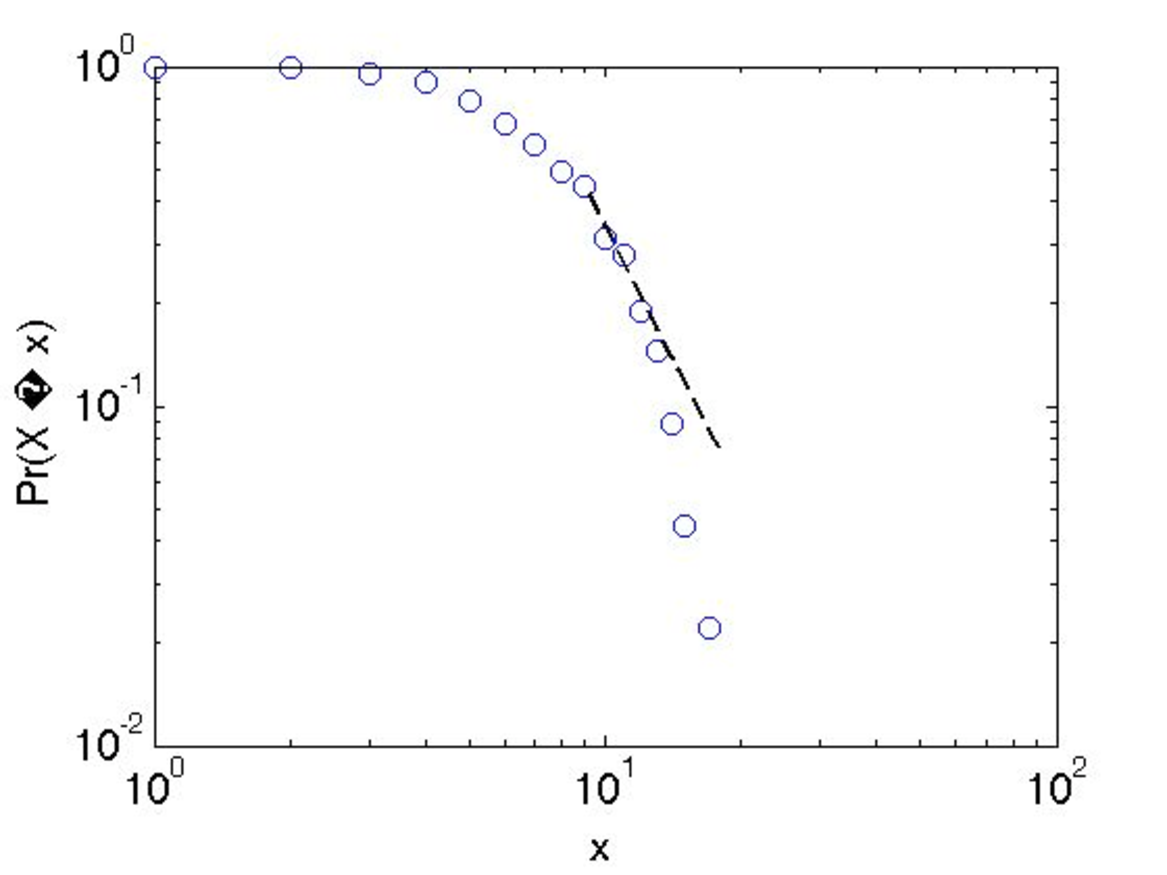
\includegraphics [scale=0.4]  {figures/PowerLawplfit.pdf}
\caption{Caption}
\label{Fig:PL}
\end{center}
\end{figure} 

\begin{figure}[!h]
\begin{center}
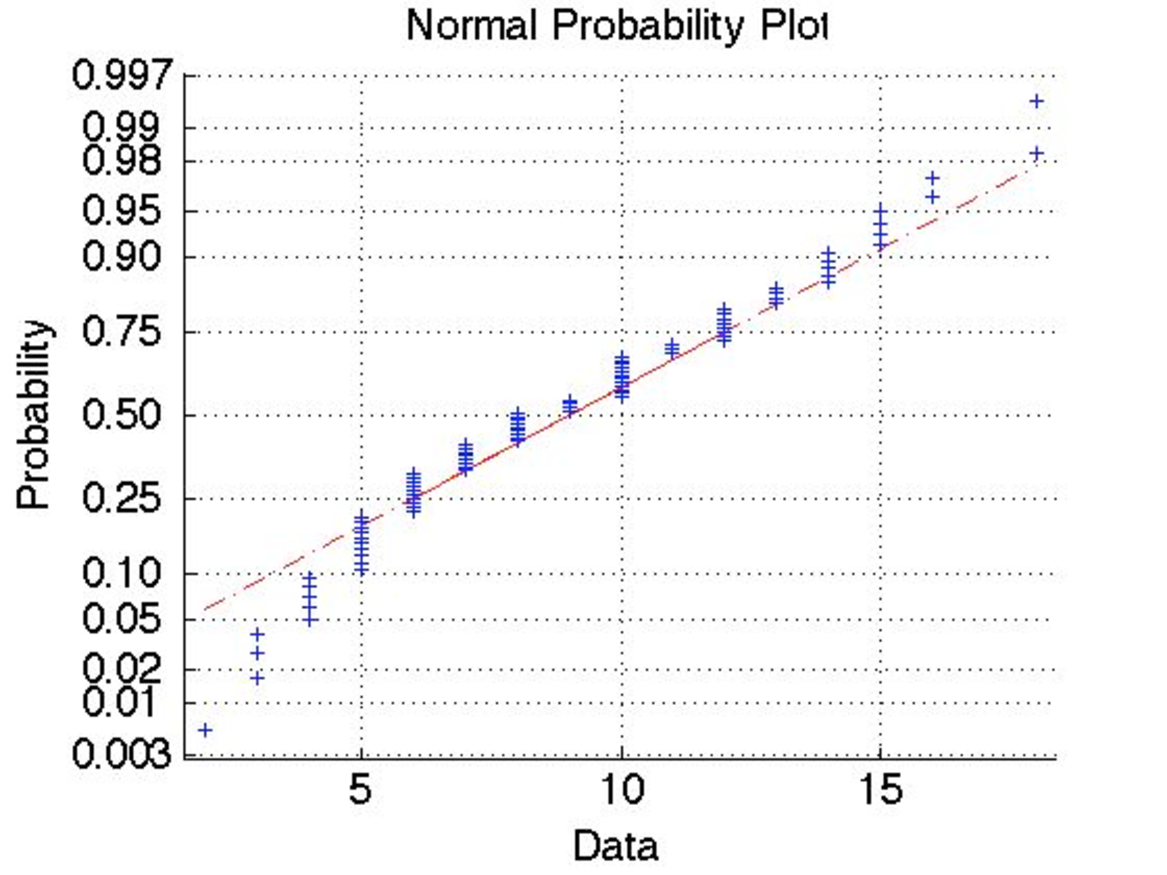
\includegraphics [scale=0.4]  {figures/Normaldistrib.pdf}
\caption{Caption}
\label{Fig:Normal}
\end{center}
\end{figure} 

%Network Identification

In order to asses the network topology of the network depicted in Figure
\ref{Fig:Pajek}we need first to determine the randomized counterpart of the
given network in order to relate the graph properties of
the original network with those of the randomly built synthetic
networks. Thus, the randomly built synthetic
networks provide the null model that we
need in order to identify whether the graph invariants in the real network are
over represented or under represented in relation with the synthetic networks. 

\begin{figure}[!h]
\begin{center}
\centerline{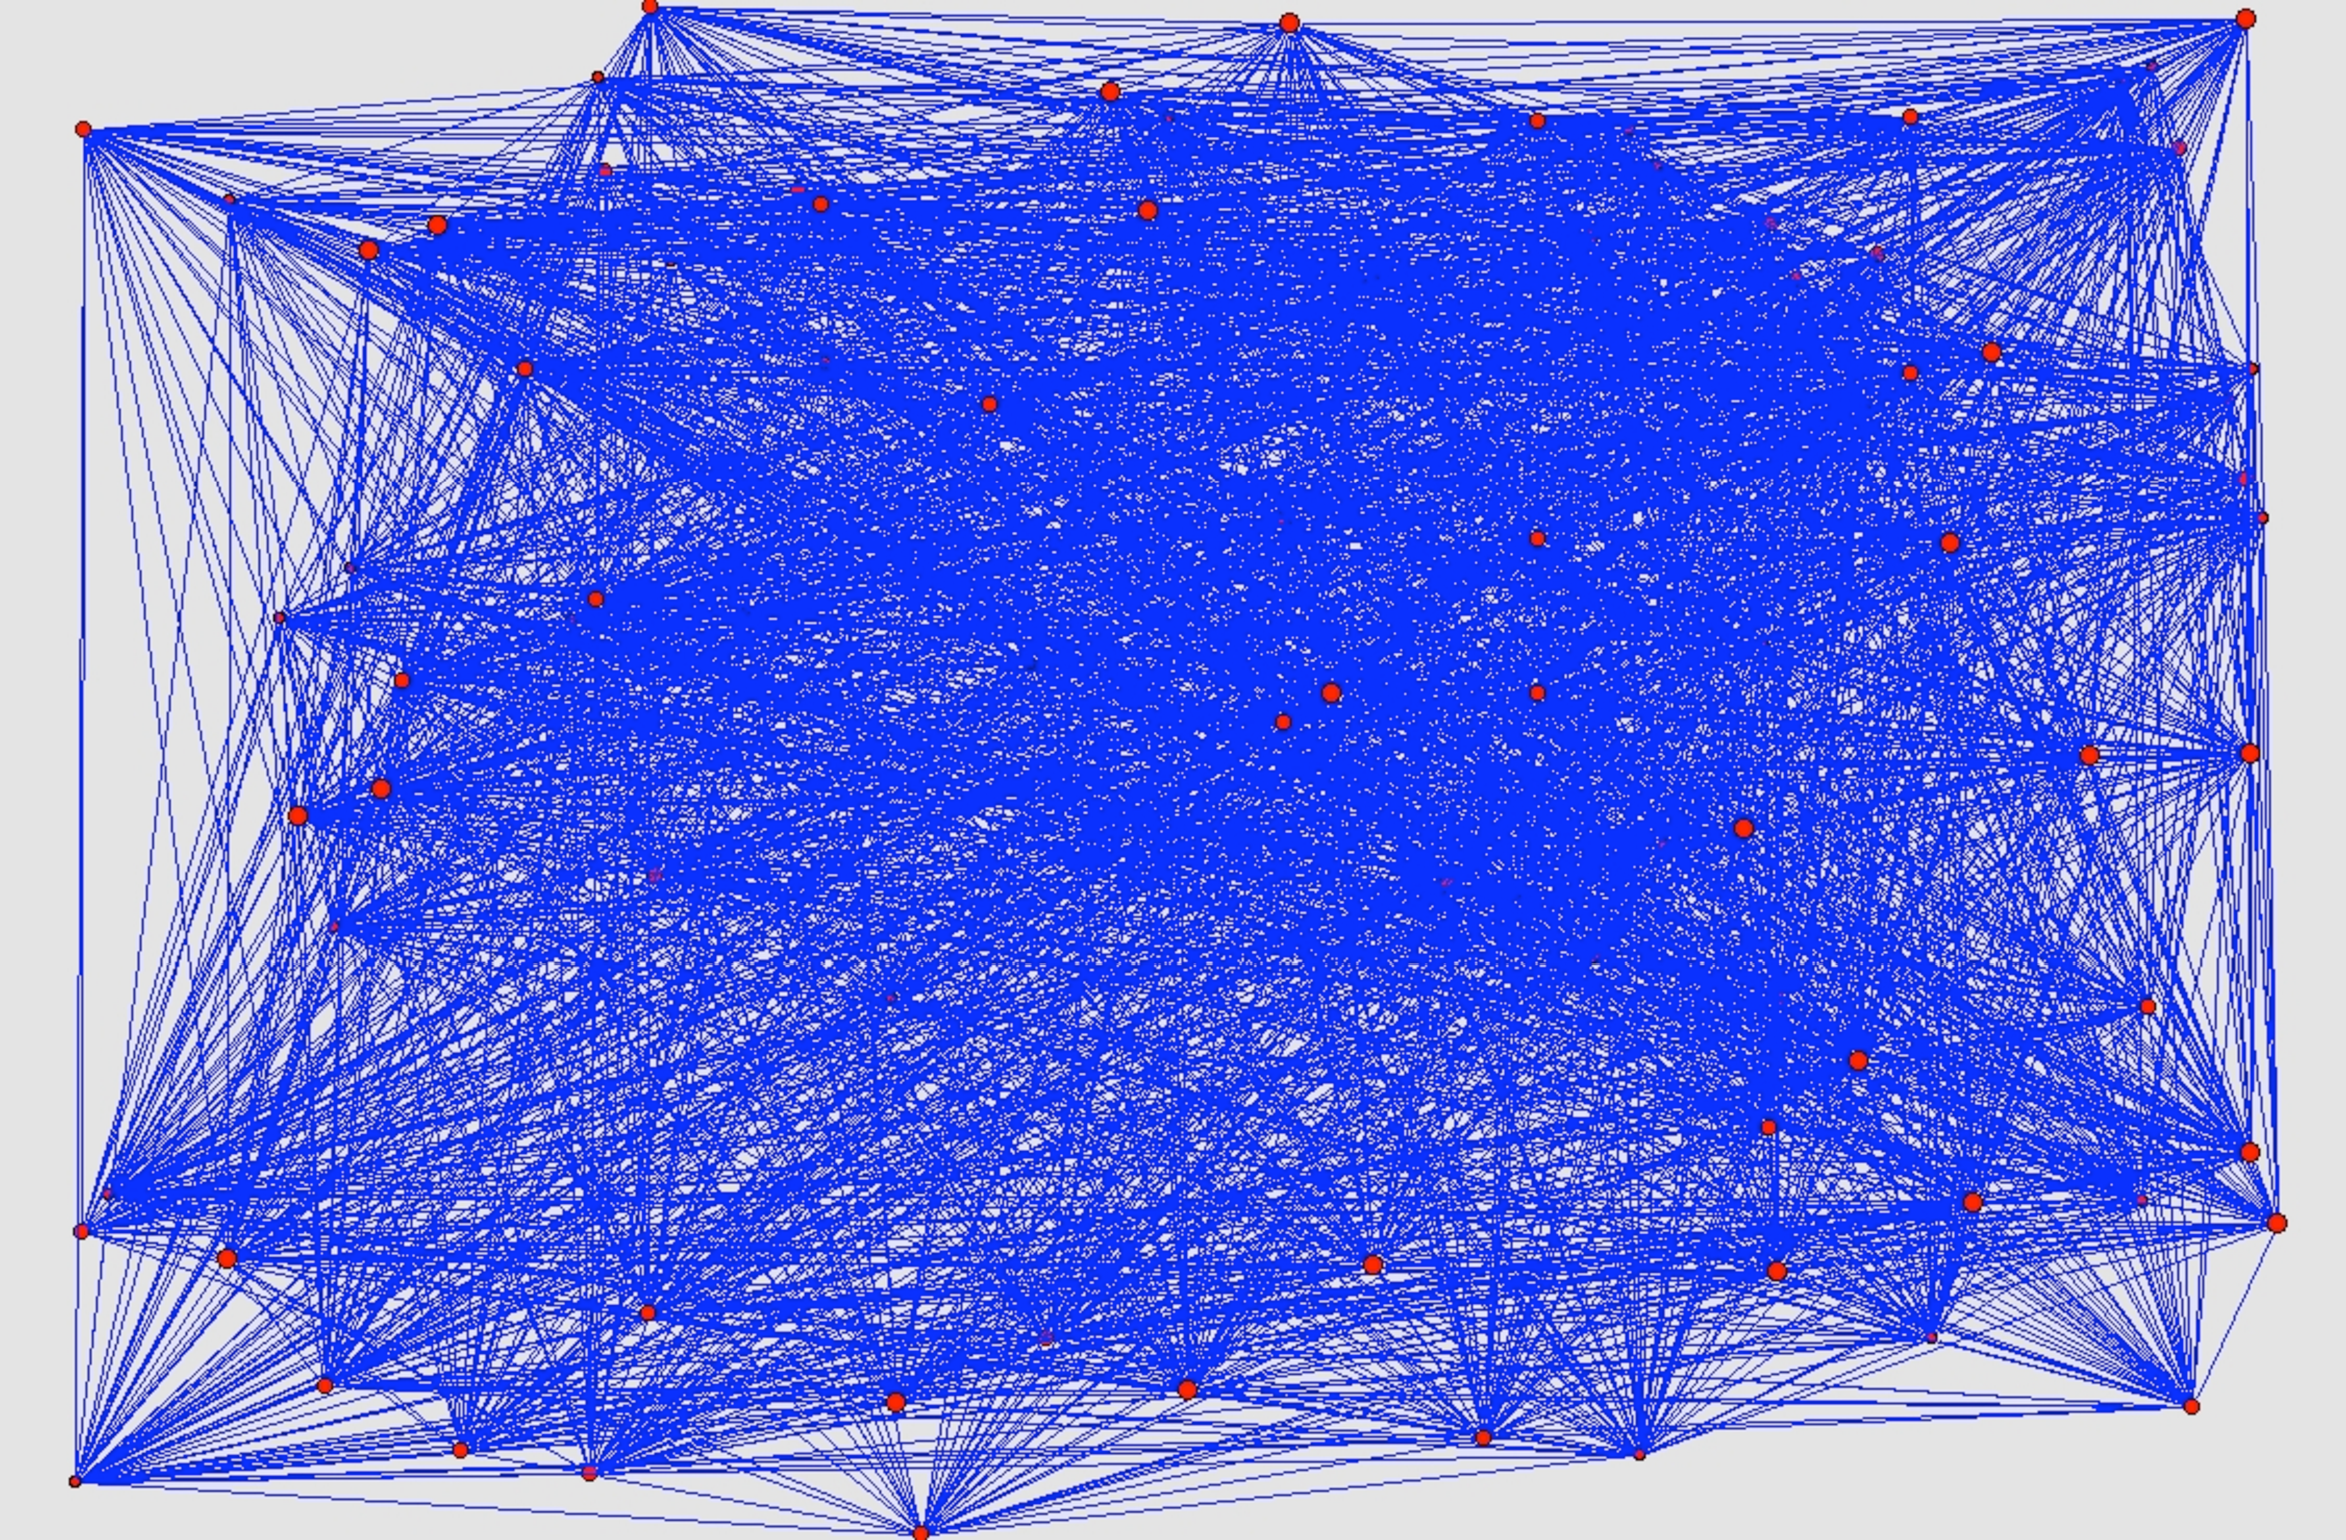
\includegraphics [scale=0.4]  {figures/Pajek9090.pdf}}
\caption{Caption Pajek}
\label{Fig:Pajek}
\end{center}
\end{figure} 

Here we explain how the generate a pool
of randomly generated random network, then we compare the metric for the real
network with this pool. 
There are a number of different algorithms that may
generate a pool of random network that maintain specific characteristics (graph
invariants) that we wish the random network hold, such as connectivity degree,
number of nodes, number of edges etc. First, we use the Renyi-Erdos model to
provide a population of random networks with the same number of nodes and edges than the
brain network (See Appendix for details).
We obtain the global path length
$\lambda= \frac{\lambda_{real}}{\lambda_{random}} =\frac{0.0881}{0.0993}
=0.8881$ and the local clustering coefficient is
$\Sigma=\frac{\Sigma_{real}}{\Sigma_{random}} =
\frac{0.7790}{0.1005}=7.7527$. Thus, $\sigma= \frac{\Sigma }{\lambda}=8.7299$,
which indicates that the clustering tin the real network is much higher than in the counterpart random networks and the
distance in the characteristic path length between the real and
the randomly generated network is close to 1.
A different alternative to create random networks is using the Maslov's
algorithm \cite{maslov_specificity_2002}. Here the degree of the nodes is
preserved, that is, each node in the generated random network will have the
same number of immediate neighbors. In the left side of Figure
\ref{Fig:Maslov}is shown the systematic deviations of the ratio
$P(K0,K1)/P(K0,K1))$ from 1, and on the right side is depicted the statistical
significance of the deviations. Both plots combined reveals regions on the
plane were connections between brain regions are significantly enhanced or
supressed compared to the null model. The red region in the left side plot
indicates the tendency of poorly connected nodes to associate with other poorly
connected nodes (less than four neighbors), blue regions in the upper left and
lower right shows the reduced likelihood that highly connected nodes are
directly linked with poorly connected nodes and viceversa. The Z scores plot on
the right of Figure \ref{Fig:Maslov} is the normalized statistical
significance of the deviations  or $Z(K0,K1) = \frac {(P(K0,K1) - P(K0,K1)} {
\sigma_ {r}(K0,K1)}$ , where $\sigma_ {r}(K0,K1)$ is the the standard deviation of
$P(K0,K1)$ in 100 realizations of a randomized network.

\begin{figure}[!h]
\begin{center}
\centerline{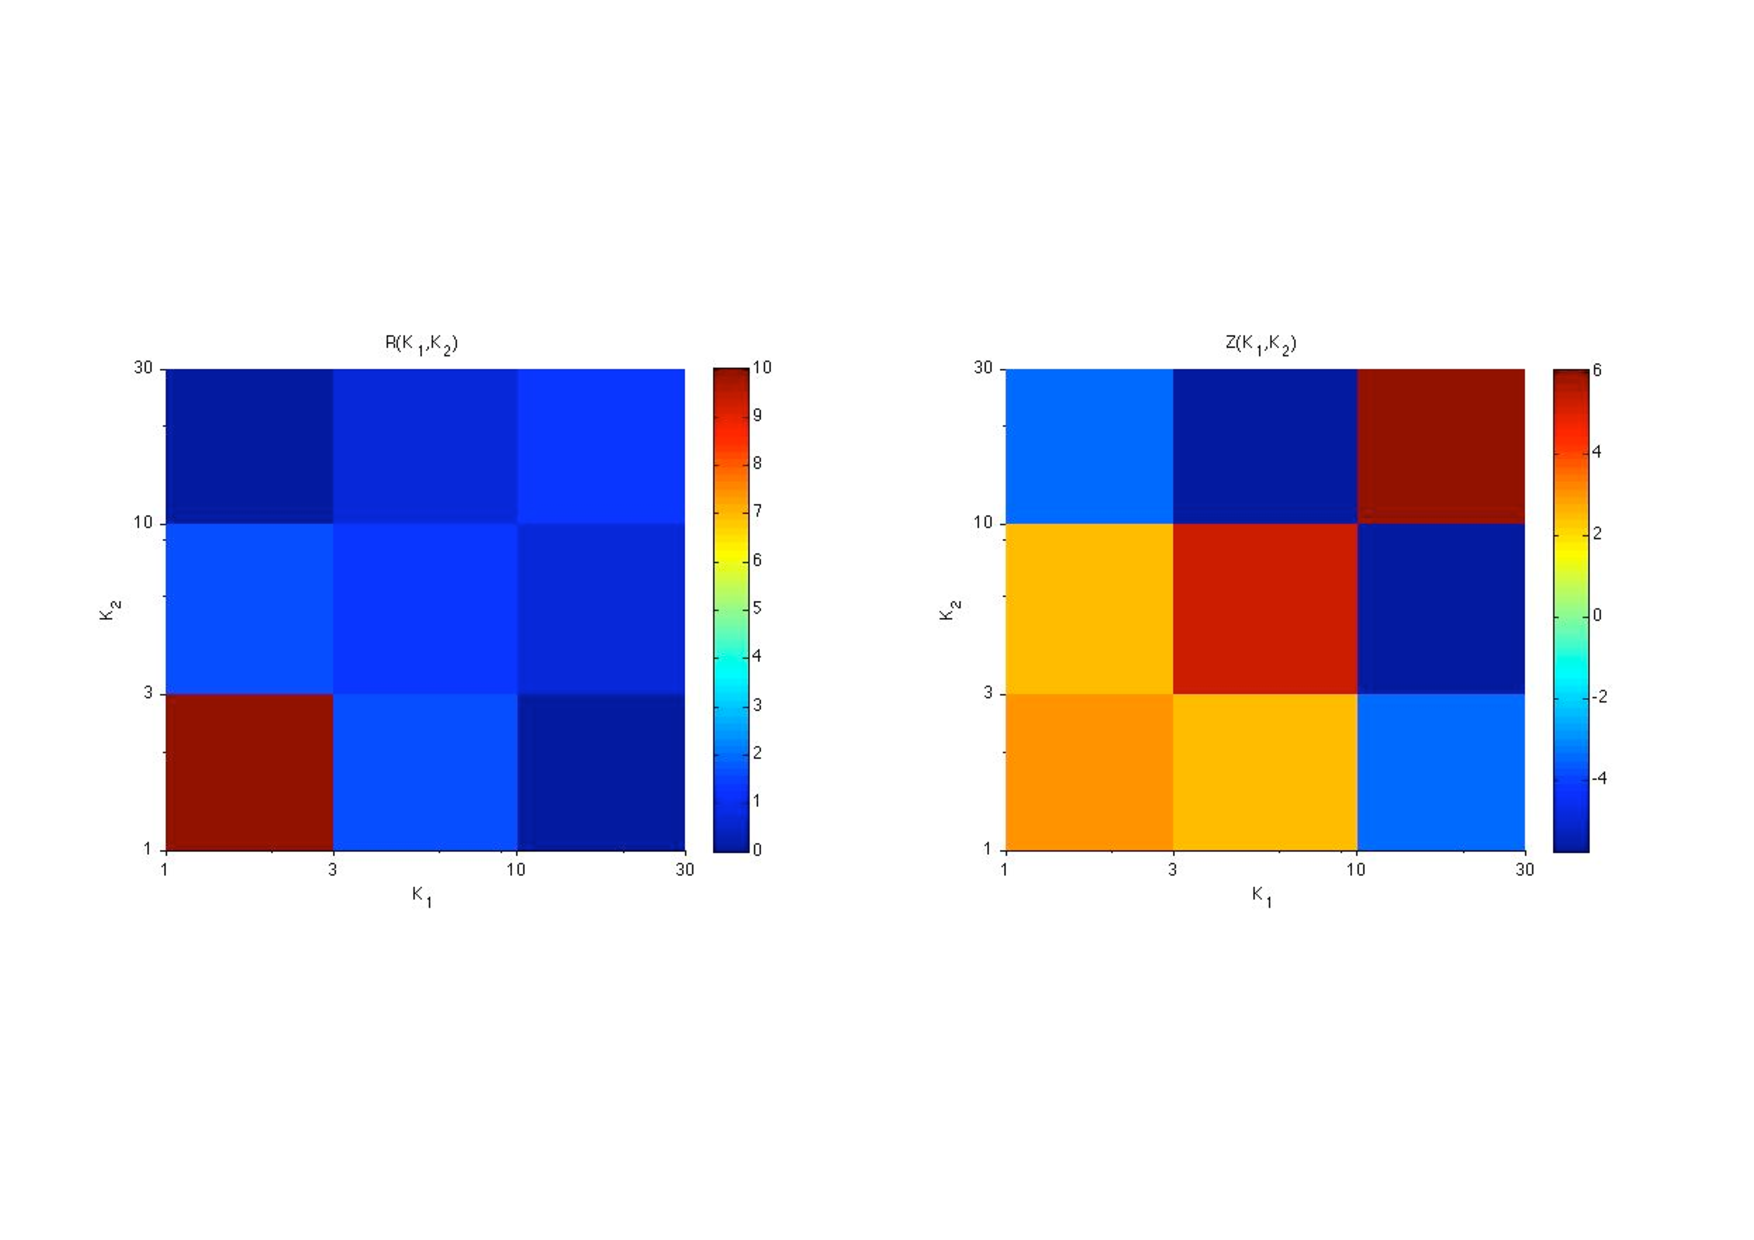
\includegraphics [scale=0.5]  {figures/MaslovRandZK1K2.pdf}}
\caption{Caption}
\label{Fig:Maslov}
\end{center}
\end{figure} 

\end{document}